\section{Technical Appendices and Supplementary Material}


\subsection{Details for Main Experiments}
\label{sec:main-experiment-details}

\subsubsection{Experiment setup details}
\label{sec:experiment-setup-details}

\paragraph{Setup of Spec-Bench experiments (Sec.~\ref{sec:baseline-comparisons}).}
We conducted our Spec-Bench experiments by running the Spec-Bench codebase from the original repository with the following modifications. First, we updated the code to work with the latest version of the \texttt{transformers} library, which is required to run recent open-source LLMs such as \texttt{meta-llama/Llama-3.1}. We also added support for arbitrary datasets (such as SWE-Bench and AgenticSQL) and implemented SuffixDecoding within the framework. We ran the experiments on a 8xH100 80GB GPU cluster, with 1TB RAM. We ran each baseline using one GPU, and a batch size of 1, just like in the original SpecBench code. 

\paragraph{Setup of vLLM SWE-Bench experiment (Sec.~\ref{sec:vllm-swebench-results}).}
We conducted the end-to-end SWE-Bench experiment on a 8xH100 80GB GPU cluster, with 1TB RAM. We served the \texttt{all-hands/openhands-lm-32b-v0.1-ep3} model locally using vLLM, with a tensor parallelism degree of 4 and with prefix caching enabled. We used the flashinfer kernels for sampling. We made some minor modifications to vLLM to record the per-request and per-step statistics of interest (time-per-token latency, throughput, acceptance length, acceptance rate). We used the same settings for all baselines. We ran the OpenHands daemon on the same machine, and used the OpenAI API to interact with the vLLM server. We ran OpenHands with the CodeActAgent~\citep{wang2024executablecodeactionselicit} with \texttt{ITERATIVE\_EVAL\_MODE=true}, and a maximum of 100 iterations, as recommended by the OpenHands authors. We used a maximum of 16 concurrent workers to run the SWE-Bench tasks.

\subsubsection{Detailed sub-task results}

The following tables present detailed performance metrics across all evaluation benchmarks. For Spec-Bench, the 13 categories include both single-turn open-ended tasks (qa, rag, math\_reasoning, summarization, translation) and multi-turn tasks. Eight of these categories (Writing, Roleplay, Reasoning, Math, Coding, Extraction, STEM, Humanities) are from MT-Bench~\citep{mtbench}, allowing direct performance comparison on this widely-used benchmark.

\textbf{SWE-Bench: Mean accepted tokens (tokens/step)}
\begin{table}[H]
\begin{adjustbox}{width=\linewidth}
\centering
\begin{tabular}{lccccccccccccc}
\toprule
\textbf{System} & astropy & django & matplotlib & seaborn & flask & requests & xarray & pylint & pytest & scikit-learn & sphinx & sympy & \textbf{Overall} \\
\midrule
suffix (linear) & 6.415 & 6.546 & 5.521 & 7.207 & 3.772 & 6.480 & 7.137 & 4.635 & 5.412 & 5.933 & 17.140 & 5.165 & 7.821 \\
suffix (tree) & 6.262 & 6.221 & 4.992 & 7.064 & 3.708 & 5.922 & 6.764 & 4.452 & 5.311 & 5.600 & 16.876 & 5.020 & 7.552 \\
pld & 2.831 & 3.008 & 2.756 & 3.080 & 2.195 & 2.996 & 3.223 & 2.629 & 2.904 & 2.669 & 4.724 & 2.641 & 3.168 \\
recycling & 3.159 & 3.058 & 3.004 & 3.133 & - & - & 2.978 & 3.072 & 2.992 & 3.046 & 2.994 & - & 3.054 \\
vanilla & 1.000 & 1.000 & 1.000 & 1.000 & 1.000 & 1.000 & 1.000 & 1.000 & 1.000 & 1.000 & 1.000 & 1.000 & 1.000 \\
eagle3 & - & - & - & - & - & - & - & - & - & - & - & - & - \\
eagle2 & - & - & - & - & - & - & - & - & - & - & - & - & - \\
eagle & - & - & - & - & - & - & - & - & - & - & - & - & - \\
hybrid & - & - & - & - & - & - & - & - & - & - & - & - & - \\
\bottomrule
\end{tabular}
\end{adjustbox}
\end{table}

\textbf{SWE-Bench: Mean Acceptance Rate}
\begin{table}[H]
\begin{adjustbox}{width=\linewidth}
\centering
\begin{tabular}{lccccccccccccc}
\toprule
\textbf{System} & astropy & django & matplotlib & seaborn & flask & requests & xarray & pylint & pytest & scikit-learn & sphinx & sympy & \textbf{Overall} \\
\midrule
suffix (linear) & 0.252 & 0.255 & 0.238 & 0.293 & 0.167 & 0.250 & 0.281 & 0.204 & 0.230 & 0.243 & 0.554 & 0.217 & 0.296 \\
suffix (tree) & 0.235 & 0.230 & 0.195 & 0.272 & 0.153 & 0.222 & 0.250 & 0.183 & 0.217 & 0.216 & 0.539 & 0.196 & 0.274 \\
pld & 0.191 & 0.210 & 0.184 & 0.215 & 0.128 & 0.208 & 0.231 & 0.174 & 0.199 & 0.175 & 0.379 & 0.175 & 0.225 \\
recycling & 0.028 & 0.027 & 0.026 & 0.028 & - & - & 0.025 & 0.027 & 0.025 & 0.026 & 0.026 & - & 0.026 \\
vanilla & - & - & - & - & - & - & - & - & - & - & - & - & - \\
suffix-1.0-tree & 0.385 & 0.381 & 0.348 & 0.420 & 0.330 & 0.388 & 0.409 & 0.349 & 0.375 & 0.375 & 0.632 & 0.373 & 0.421 \\
\bottomrule
\end{tabular}
\end{adjustbox}
\end{table}

\textbf{SWE-Bench: Time per output token (ms)}
\begin{table}[H]
\begin{adjustbox}{width=\linewidth}
\centering
\begin{tabular}{lccccccccccccc}
\toprule
\textbf{System} & astropy & django & matplotlib & seaborn & flask & requests & xarray & pylint & pytest & scikit-learn & sphinx & sympy & \textbf{Overall} \\
\midrule
suffix (linear) & 30.563 & 21.881 & 26.013 & 37.012 & 22.238 & 23.828 & 23.598 & 27.739 & 29.313 & 31.949 & 25.613 & 17.072 & 27.436 \\
suffix (tree) & 30.800 & 22.238 & 26.278 & 37.095 & 22.728 & 23.998 & 23.847 & 28.388 & 29.451 & 32.496 & 25.853 & 17.199 & 27.711 \\
pld & 41.675 & 31.029 & 34.447 & 47.588 & 31.549 & 31.155 & 31.330 & 37.386 & 38.238 & 41.531 & 41.877 & 25.142 & 37.758 \\
recycling & 41.328 & 31.847 & 34.155 & 49.670 & - & - & 33.434 & 34.304 & 38.438 & 39.667 & 78.153 & - & 43.774 \\
vanilla & 50.080 & 41.102 & 43.019 & 57.069 & 35.040 & 39.268 & 41.213 & 42.107 & 45.633 & 46.061 & 77.815 & 32.527 & 50.074 \\
eagle3 & - & - & - & - & - & - & - & - & - & - & - & - & - \\
eagle2 & - & - & - & - & - & - & - & - & - & - & - & - & - \\
eagle & - & - & - & - & - & - & - & - & - & - & - & - & - \\
hybrid & - & - & - & - & - & - & - & - & - & - & - & - & - \\
\bottomrule
\end{tabular}
\end{adjustbox}
\end{table}

\textbf{SWE-Bench: Speculation time per generated token (ms)}
\begin{table}[H]
\begin{adjustbox}{width=\linewidth}
\centering
\begin{tabular}{lccccccccccccc}
\toprule
\textbf{System} & astropy & django & matplotlib & seaborn & flask & requests & xarray & pylint & pytest & scikit-learn & sphinx & sympy & \textbf{Overall} \\
\midrule
vanilla & 0.000 & 0.000 & 0.000 & 0.000 & 0.000 & 0.000 & 0.000 & 0.000 & 0.000 & 0.000 & 0.000 & 0.000 & 0.000 \\
suffix (linear) & 0.156 & 0.122 & 0.175 & 0.185 & 0.198 & 0.182 & 0.178 & 0.203 & 0.217 & 0.203 & 0.125 & 0.167 & 0.171 \\
suffix (tree) & 0.170 & 0.135 & 0.172 & 0.172 & 0.191 & 0.165 & 0.165 & 0.235 & 0.235 & 0.212 & 0.138 & 0.150 & 0.175 \\
pld & 0.191 & 0.197 & 0.208 & 0.176 & 0.266 & 0.200 & 0.191 & 0.222 & 0.208 & 0.228 & 0.126 & 0.217 & 0.191 \\
recycling & 9.298 & 6.023 & 7.982 & 13.731 & - & - & 6.607 & 7.665 & 8.081 & 11.748 & 19.653 & - & 10.582 \\
eagle3 & - & - & - & - & - & - & - & - & - & - & - & - & - \\
eagle2 & - & - & - & - & - & - & - & - & - & - & - & - & - \\
eagle & - & - & - & - & - & - & - & - & - & - & - & - & - \\
hybrid & - & - & - & - & - & - & - & - & - & - & - & - & - \\
\bottomrule
\end{tabular}
\end{adjustbox}
\end{table}

\textbf{SWE-Bench: Speedup over vanilla decoding}
\begin{table}[H]
\begin{adjustbox}{width=\linewidth}
\centering
\begin{tabular}{lccccccccccccc}
\toprule
\textbf{System} & astropy & django & matplotlib & seaborn & flask & requests & xarray & pylint & pytest & scikit-learn & sphinx & sympy & \textbf{Overall} \\
\midrule
suffix (linear) & 2.213 & 2.442 & 2.039 & 1.951 & 1.792 & 1.962 & 2.210 & 1.792 & 1.888 & 2.356 & 4.453 & 2.292 & 2.452 \\
suffix (tree) & 2.158 & 2.412 & 1.991 & 1.985 & 1.759 & 1.972 & 2.190 & 1.754 & 1.912 & 2.296 & 4.417 & 2.280 & 2.433 \\
pld & 1.440 & 1.516 & 1.425 & 1.360 & 1.242 & 1.399 & 1.486 & 1.270 & 1.326 & 1.429 & 2.006 & 1.483 & 1.495 \\
recycling & 1.427 & 1.458 & 1.483 & 1.264 & - & - & 1.360 & 1.311 & 1.290 & 1.399 & 1.328 & - & 1.358 \\
vanilla & 1.000 & 1.000 & 1.000 & 1.000 & 1.000 & 1.000 & 1.000 & 1.000 & 1.000 & 1.000 & 1.000 & 1.000 & 1.000 \\
eagle3 & - & - & - & - & - & - & - & - & - & - & - & - & - \\
eagle2 & - & - & - & - & - & - & - & - & - & - & - & - & - \\
eagle & - & - & - & - & - & - & - & - & - & - & - & - & - \\
hybrid & - & - & - & - & - & - & - & - & - & - & - & - & - \\
\bottomrule
\end{tabular}
\end{adjustbox}
\end{table}

\textbf{AgenticSQL: Mean accepted tokens (tokens/step)}
\begin{table}[H]
\begin{adjustbox}{width=\linewidth}
\centering
\begin{tabular}{lcccccccc}
\toprule
\textbf{System} & Classify & Extract & Enrich & Combine & SQL1 & SQL2 & SQL3 & \textbf{Overall} \\
\midrule
hybrid (tree) & 4.180 & 14.813 & 15.081 & 6.448 & 3.983 & 3.932 & 4.006 & 7.500 \\
hybrid (linear) & 4.008 & 13.473 & 15.304 & 6.362 & 3.876 & 3.842 & 3.913 & 7.262 \\
suffix (linear) & 3.577 & 11.833 & 12.395 & 5.924 & 3.665 & 3.005 & 4.005 & 6.349 \\
suffix (tree) & 3.470 & 11.724 & 12.137 & 5.834 & 3.633 & 2.914 & 3.904 & 6.236 \\
eagle2 & 3.156 & 5.173 & 3.249 & 3.534 & 3.066 & 3.761 & 3.057 & 3.572 \\
recycling & 2.915 & 4.125 & 3.125 & 3.138 & 2.951 & 2.929 & 2.994 & 3.169 \\
eagle3 & 2.529 & 3.374 & 4.198 & 3.179 & 2.142 & 4.622 & 2.056 & 3.160 \\
eagle & 2.305 & 4.062 & 2.877 & 3.127 & 2.166 & 3.295 & 2.109 & 2.851 \\
pld & 1.427 & 4.134 & 1.455 & 3.914 & 2.074 & 1.452 & 2.151 & 2.373 \\
vanilla & 1.000 & 1.000 & 1.000 & 1.000 & 1.000 & 1.000 & 1.000 & 1.000 \\
\bottomrule
\end{tabular}
\end{adjustbox}
\end{table}

\textbf{AgenticSQL: Mean Acceptance Rate}
\begin{table}[H]
\begin{adjustbox}{width=\linewidth}
\centering
\begin{tabular}{lcccccccc}
\toprule
\textbf{System} & Classify & Extract & Enrich & Combine & SQL1 & SQL2 & SQL3 & \textbf{Overall} \\
\midrule
vanilla & - & - & - & - & - & - & - & - \\
suffix (linear) & 0.212 & 0.628 & 0.740 & 0.428 & 0.318 & 0.245 & 0.330 & 0.415 \\
suffix (tree) & 0.189 & 0.605 & 0.614 & 0.397 & 0.294 & 0.225 & 0.298 & 0.375 \\
hybrid (tree) & 0.131 & 0.642 & 0.683 & 0.249 & 0.138 & 0.143 & 0.140 & 0.304 \\
hybrid (linear) & 0.124 & 0.595 & 0.750 & 0.242 & 0.130 & 0.139 & 0.133 & 0.302 \\
pld & 0.061 & 0.365 & 0.069 & 0.355 & 0.137 & 0.076 & 0.144 & 0.173 \\
eagle & 0.052 & 0.122 & 0.075 & 0.085 & 0.047 & 0.092 & 0.044 & 0.074 \\
eagle2 & 0.036 & 0.070 & 0.037 & 0.042 & 0.034 & 0.046 & 0.034 & 0.043 \\
eagle3 & 0.025 & 0.040 & 0.053 & 0.036 & 0.019 & 0.060 & 0.018 & 0.036 \\
recycling & 0.025 & 0.041 & 0.028 & 0.027 & 0.025 & 0.024 & 0.026 & 0.028 \\
\bottomrule
\end{tabular}
\end{adjustbox}
\end{table}

\textbf{AgenticSQL: Time per output token (ms)}
\begin{table}[H]
\begin{adjustbox}{width=\linewidth}
\centering
\begin{tabular}{lcccccccc}
\toprule
\textbf{System} & Classify & Extract & Enrich & Combine & SQL1 & SQL2 & SQL3 & \textbf{Overall} \\
\midrule
suffix (linear) & 9.552 & 2.687 & 3.007 & 6.023 & 9.559 & 10.588 & 9.767 & 7.306 \\
suffix (tree) & 9.594 & 2.876 & 3.188 & 6.164 & 10.339 & 10.935 & 10.090 & 7.592 \\
hybrid (tree) & 11.975 & 3.491 & 3.633 & 7.883 & 14.329 & 11.600 & 14.399 & 9.604 \\
recycling & 10.316 & 7.314 & 9.470 & 9.724 & 10.981 & 9.981 & 10.702 & 9.782 \\
hybrid (linear) & 12.563 & 3.681 & 3.762 & 8.603 & 14.827 & 11.639 & 21.219 & 10.874 \\
eagle2 & 16.814 & 9.210 & 15.078 & 13.877 & 17.967 & 12.312 & 17.531 & 14.677 \\
pld & 20.146 & 7.735 & 20.321 & 8.173 & 14.605 & 20.546 & 14.646 & 15.169 \\
eagle & 21.221 & 11.308 & 15.760 & 15.688 & 23.353 & 13.396 & 24.595 & 17.887 \\
eagle3 & 23.334 & 14.729 & 12.513 & 16.863 & 26.997 & 10.747 & 27.728 & 18.966 \\
vanilla & 26.578 & 25.292 & 25.032 & 25.406 & 27.011 & 25.851 & 26.307 & 25.924 \\
\bottomrule
\end{tabular}
\end{adjustbox}
\end{table}

\textbf{AgenticSQL: Speculation time per generated token (ms)}
\begin{table}[H]
\begin{adjustbox}{width=\linewidth}
\centering
\begin{tabular}{lcccccccc}
\toprule
\textbf{System} & Classify & Extract & Enrich & Combine & SQL1 & SQL2 & SQL3 & \textbf{Overall} \\
\midrule
vanilla & 0.000 & 0.000 & 0.000 & 0.000 & 0.000 & 0.000 & 0.000 & 0.000 \\
suffix (linear) & 0.060 & 0.015 & 0.015 & 0.033 & 0.059 & 0.058 & 0.061 & 0.043 \\
suffix (tree) & 0.064 & 0.017 & 0.020 & 0.035 & 0.064 & 0.062 & 0.064 & 0.047 \\
pld & 0.419 & 0.124 & 0.422 & 0.130 & 0.281 & 0.434 & 0.276 & 0.298 \\
recycling & 0.762 & 0.303 & 0.399 & 0.577 & 0.928 & 0.260 & 0.922 & 0.592 \\
hybrid (tree) & 1.728 & 0.249 & 0.376 & 1.112 & 2.350 & 0.927 & 2.372 & 1.299 \\
hybrid (linear) & 1.776 & 0.256 & 0.358 & 1.177 & 2.387 & 0.930 & 4.389 & 1.604 \\
eagle & 3.189 & 1.693 & 2.423 & 2.372 & 3.423 & 2.197 & 3.616 & 2.700 \\
eagle2 & 4.118 & 2.006 & 3.292 & 3.308 & 4.599 & 2.597 & 4.509 & 3.487 \\
eagle3 & 6.092 & 3.526 & 3.021 & 4.350 & 7.156 & 2.543 & 7.332 & 4.854 \\
\bottomrule
\end{tabular}
\end{adjustbox}
\end{table}

\textbf{AgenticSQL: Speedup over vanilla decoding}
\begin{table}[H]
\begin{adjustbox}{width=\linewidth}
\centering
\begin{tabular}{lcccccccc}
\toprule
\textbf{System} & Classify & Extract & Enrich & Combine & SQL1 & SQL2 & SQL3 & \textbf{Overall} \\
\midrule
suffix (linear) & 3.016 & 9.854 & 10.406 & 4.848 & 3.205 & 2.839 & 3.211 & 5.345 \\
suffix (tree) & 2.998 & 9.545 & 10.009 & 4.765 & 3.008 & 2.733 & 3.133 & 5.175 \\
hybrid (tree) & 2.338 & 7.672 & 8.191 & 3.613 & 2.057 & 2.496 & 2.077 & 4.068 \\
hybrid (linear) & 2.243 & 7.137 & 7.965 & 3.327 & 1.993 & 2.483 & 1.405 & 3.799 \\
recycling & 2.588 & 3.472 & 2.672 & 2.640 & 2.502 & 2.604 & 2.492 & 2.710 \\
pld & 1.330 & 3.695 & 1.255 & 3.298 & 1.936 & 1.311 & 1.905 & 2.105 \\
eagle2 & 1.591 & 2.751 & 1.673 & 1.855 & 1.527 & 2.119 & 1.527 & 1.864 \\
eagle3 & 1.328 & 1.720 & 2.025 & 1.619 & 1.108 & 2.496 & 1.056 & 1.623 \\
eagle & 1.324 & 2.246 & 1.598 & 1.669 & 1.229 & 1.955 & 1.138 & 1.595 \\
vanilla & 1.000 & 1.000 & 1.000 & 1.000 & 1.000 & 1.000 & 1.000 & 1.000 \\
\bottomrule
\end{tabular}
\end{adjustbox}
\end{table}

\textbf{Spec-Bench: Mean accepted tokens (tokens/step)}
\begin{table}[H]
\begin{adjustbox}{width=\linewidth}
\centering
\begin{tabular}{lcccccccccccccc}
\toprule
\textbf{System} & coding & extraction & humanities & math & math\_reasoning & qa & rag & reasoning & roleplay & stem & summarization & translation & writing & \textbf{Overall} \\
\midrule
hybrid (tree) & 6.325 & 5.418 & 4.980 & 5.817 & 5.080 & 4.958 & 4.812 & 4.610 & 4.556 & 5.155 & 4.550 & 3.432 & 5.306 & 4.684 \\
eagle3 & 5.975 & 5.373 & 5.180 & 5.745 & 5.562 & 4.351 & 5.009 & 4.956 & 4.664 & 5.299 & 4.767 & 2.909 & 5.093 & 4.647 \\
hybrid (linear) & 5.958 & 5.249 & 4.966 & 5.446 & 5.121 & 4.452 & 4.753 & 4.607 & 4.557 & 5.089 & 4.520 & 3.345 & 5.158 & 4.553 \\
eagle2 & 4.766 & 3.842 & 3.612 & 4.242 & 4.129 & 3.324 & 3.630 & 3.892 & 3.353 & 3.736 & 3.254 & 2.605 & 3.383 & 3.466 \\
eagle & 4.149 & 3.469 & 3.177 & 3.724 & 3.617 & 2.857 & 3.239 & 3.328 & 2.968 & 3.311 & 2.926 & 2.352 & 3.082 & 3.065 \\
recycling & 3.044 & 2.610 & 2.539 & 3.128 & 2.980 & 2.372 & 2.352 & 2.537 & 2.338 & 2.697 & 2.614 & 2.305 & 2.417 & 2.548 \\
suffix (linear) & 1.981 & 1.757 & 1.454 & 2.161 & 1.661 & 1.878 & 1.999 & 1.521 & 1.252 & 1.485 & 1.725 & 1.705 & 1.435 & 1.766 \\
suffix (tree) & 1.960 & 1.754 & 1.461 & 2.134 & 1.638 & 1.874 & 1.957 & 1.504 & 1.259 & 1.501 & 1.703 & 1.705 & 1.424 & 1.750 \\
pld & 1.911 & 1.670 & 1.387 & 1.957 & 1.475 & 1.461 & 1.967 & 1.490 & 1.206 & 1.430 & 1.816 & 1.362 & 1.394 & 1.606 \\
vanilla & 1.000 & 1.000 & 1.000 & 1.000 & 1.000 & 1.000 & 1.000 & 1.000 & 1.000 & 1.000 & 1.000 & 1.000 & 1.000 & 1.000 \\
\bottomrule
\end{tabular}
\end{adjustbox}
\end{table}

\textbf{Spec-Bench: Mean Acceptance Rate}
\begin{table}[H]
\begin{adjustbox}{width=\linewidth}
\centering
\begin{tabular}{lcccccccccccccc}
\toprule
\textbf{System} & coding & extraction & humanities & math & math\_reasoning & qa & rag & reasoning & roleplay & stem & summarization & translation & writing & \textbf{Overall} \\
\midrule
suffix (linear) & 0.255 & 0.216 & 0.162 & 0.240 & 0.163 & 0.152 & 0.216 & 0.171 & 0.116 & 0.169 & 0.199 & 0.216 & 0.208 & 0.190 \\
vanilla & - & - & - & - & - & - & - & - & - & - & - & - & - & - \\
suffix (tree) & 0.244 & 0.211 & 0.156 & 0.232 & 0.149 & 0.144 & 0.203 & 0.156 & 0.115 & 0.165 & 0.189 & 0.208 & 0.194 & 0.179 \\
pld & 0.132 & 0.097 & 0.063 & 0.126 & 0.071 & 0.088 & 0.119 & 0.076 & 0.037 & 0.068 & 0.103 & 0.130 & 0.072 & 0.099 \\
eagle & 0.126 & 0.099 & 0.087 & 0.109 & 0.105 & 0.074 & 0.090 & 0.093 & 0.079 & 0.092 & 0.077 & 0.054 & 0.083 & 0.083 \\
hybrid (linear) & 0.109 & 0.084 & 0.072 & 0.100 & 0.078 & 0.074 & 0.075 & 0.069 & 0.062 & 0.075 & 0.068 & 0.044 & 0.077 & 0.070 \\
hybrid (tree) & 0.107 & 0.084 & 0.072 & 0.101 & 0.077 & 0.075 & 0.074 & 0.069 & 0.062 & 0.076 & 0.068 & 0.045 & 0.077 & 0.070 \\
eagle3 & 0.083 & 0.073 & 0.070 & 0.079 & 0.076 & 0.056 & 0.067 & 0.066 & 0.061 & 0.072 & 0.063 & 0.032 & 0.068 & 0.061 \\
eagle2 & 0.063 & 0.047 & 0.044 & 0.054 & 0.052 & 0.039 & 0.044 & 0.048 & 0.039 & 0.046 & 0.038 & 0.027 & 0.040 & 0.041 \\
recycling & 0.026 & 0.020 & 0.019 & 0.027 & 0.025 & 0.017 & 0.017 & 0.020 & 0.017 & 0.021 & 0.020 & 0.017 & 0.018 & 0.020 \\
\bottomrule
\end{tabular}
\end{adjustbox}
\end{table}

\textbf{Spec-Bench: Time per output token (ms)}
\begin{table}[H]
\begin{adjustbox}{width=\linewidth}
\centering
\begin{tabular}{lcccccccccccccc}
\toprule
\textbf{System} & coding & extraction & humanities & math & math\_reasoning & qa & rag & reasoning & roleplay & stem & summarization & translation & writing & \textbf{Overall} \\
\midrule
hybrid (linear) & 7.218 & 9.235 & 8.970 & 7.974 & 8.783 & 11.534 & 10.576 & 9.899 & 10.195 & 8.698 & 9.857 & 14.858 & 8.806 & 10.747 \\
hybrid (tree) & 7.251 & 9.588 & 9.519 & 8.203 & 9.194 & 11.880 & 11.098 & 10.543 & 10.775 & 9.133 & 10.214 & 15.262 & 9.141 & 11.153 \\
recycling & 9.475 & 11.528 & 11.333 & 9.224 & 9.749 & 13.475 & 12.957 & 11.489 & 12.425 & 10.691 & 11.373 & 13.104 & 12.019 & 11.947 \\
eagle2 & 9.721 & 13.256 & 12.822 & 11.157 & 11.338 & 14.903 & 14.012 & 12.631 & 14.229 & 12.461 & 14.422 & 19.116 & 13.992 & 14.387 \\
eagle & 10.201 & 13.193 & 13.570 & 11.485 & 11.895 & 16.219 & 14.222 & 13.215 & 14.639 & 13.022 & 14.840 & 19.425 & 14.280 & 14.925 \\
suffix (tree) & 13.833 & 16.284 & 18.670 & 13.547 & 16.304 & 19.839 & 15.285 & 18.382 & 21.339 & 18.034 & 15.825 & 16.595 & 19.154 & 16.875 \\
suffix (linear) & 13.595 & 16.245 & 18.212 & 13.292 & 16.447 & 19.999 & 15.378 & 18.061 & 21.217 & 18.041 & 15.925 & 16.670 & 18.925 & 16.936 \\
pld & 14.681 & 17.524 & 20.469 & 14.450 & 19.179 & 22.693 & 16.383 & 19.173 & 23.300 & 19.714 & 15.949 & 22.214 & 20.438 & 19.190 \\
vanilla & 24.721 & 24.903 & 24.979 & 24.466 & 24.992 & 25.082 & 25.698 & 24.475 & 24.433 & 24.871 & 25.114 & 24.904 & 24.463 & 25.076 \\
\bottomrule
\end{tabular}
\end{adjustbox}
\end{table}

\textbf{Spec-Bench: Speculation time per generated token (ms)}
\begin{table}[H]
\begin{adjustbox}{width=\linewidth}
\centering
\begin{tabular}{lcccccccccccccc}
\toprule
\textbf{System} & coding & extraction & humanities & math & math\_reasoning & qa & rag & reasoning & roleplay & stem & summarization & translation & writing & \textbf{Overall} \\
\midrule
vanilla & 0.000 & 0.000 & 0.000 & 0.000 & 0.000 & 0.000 & 0.000 & 0.000 & 0.000 & 0.000 & 0.000 & 0.000 & 0.000 & 0.000 \\
suffix (linear) & 0.071 & 0.079 & 0.099 & 0.067 & 0.087 & 0.097 & 0.089 & 0.084 & 0.101 & 0.094 & 0.092 & 0.076 & 0.084 & 0.088 \\
suffix (tree) & 0.074 & 0.080 & 0.104 & 0.069 & 0.091 & 0.099 & 0.093 & 0.088 & 0.103 & 0.097 & 0.096 & 0.079 & 0.086 & 0.091 \\
recycling & 0.243 & 0.318 & 0.291 & 0.240 & 0.255 & 0.391 & 0.419 & 0.304 & 0.320 & 0.275 & 0.321 & 0.365 & 0.310 & 0.340 \\
pld & 0.291 & 0.357 & 0.421 & 0.277 & 0.392 & 0.480 & 0.326 & 0.391 & 0.492 & 0.407 & 0.325 & 0.466 & 0.428 & 0.395 \\
hybrid (linear) & 1.369 & 1.838 & 2.026 & 1.510 & 1.854 & 2.455 & 2.152 & 2.070 & 2.353 & 1.925 & 2.118 & 3.096 & 1.949 & 2.259 \\
eagle & 1.698 & 1.977 & 2.268 & 1.877 & 1.892 & 2.389 & 2.034 & 2.060 & 2.421 & 2.166 & 2.434 & 2.885 & 2.351 & 2.289 \\
hybrid (tree) & 1.445 & 1.935 & 2.152 & 1.580 & 1.947 & 2.553 & 2.238 & 2.196 & 2.506 & 2.010 & 2.200 & 3.141 & 2.056 & 2.344 \\
eagle3 & 1.913 & 2.172 & 2.218 & 2.001 & 2.030 & 2.674 & 2.419 & 2.334 & 2.500 & 2.160 & 2.402 & 4.084 & 2.237 & 2.634 \\
eagle2 & 2.055 & 2.656 & 2.714 & 2.338 & 2.346 & 2.962 & 2.807 & 2.584 & 2.997 & 2.628 & 3.062 & 3.826 & 2.946 & 2.936 \\
\bottomrule
\end{tabular}
\end{adjustbox}
\end{table}

\textbf{Spec-Bench: Speedup over vanilla decoding}
\begin{table}[H]
\begin{adjustbox}{width=\linewidth}
\centering
\begin{tabular}{lcccccccccccccc}
\toprule
\textbf{System} & coding & extraction & humanities & math & math\_reasoning & qa & rag & reasoning & roleplay & stem & summarization & translation & writing & \textbf{Overall} \\
\midrule
hybrid (linear) & 3.441 & 2.795 & 2.800 & 3.139 & 2.866 & 2.404 & 2.542 & 2.496 & 2.461 & 2.871 & 2.573 & 1.759 & 2.833 & 2.500 \\
hybrid (tree) & 3.442 & 2.717 & 2.644 & 3.132 & 2.736 & 2.611 & 2.445 & 2.344 & 2.330 & 2.732 & 2.485 & 1.713 & 2.736 & 2.458 \\
eagle3 & 3.115 & 2.634 & 2.713 & 2.910 & 2.888 & 2.172 & 2.474 & 2.446 & 2.394 & 2.764 & 2.520 & 1.447 & 2.622 & 2.367 \\
recycling & 2.619 & 2.234 & 2.209 & 2.660 & 2.577 & 1.951 & 2.057 & 2.150 & 1.979 & 2.334 & 2.218 & 1.932 & 2.057 & 2.169 \\
eagle2 & 2.548 & 1.998 & 1.958 & 2.215 & 2.220 & 1.733 & 1.877 & 1.968 & 1.751 & 2.007 & 1.756 & 1.336 & 1.791 & 1.825 \\
eagle & 2.427 & 1.956 & 1.848 & 2.142 & 2.112 & 1.600 & 1.841 & 1.871 & 1.703 & 1.922 & 1.702 & 1.305 & 1.753 & 1.752 \\
suffix (tree) & 1.796 & 1.620 & 1.350 & 1.930 & 1.558 & 1.785 & 1.886 & 1.364 & 1.149 & 1.389 & 1.624 & 1.627 & 1.310 & 1.661 \\
suffix (linear) & 1.828 & 1.630 & 1.383 & 1.967 & 1.544 & 1.773 & 1.890 & 1.389 & 1.156 & 1.386 & 1.618 & 1.618 & 1.327 & 1.659 \\
pld & 1.712 & 1.484 & 1.231 & 1.753 & 1.323 & 1.326 & 1.807 & 1.320 & 1.055 & 1.275 & 1.628 & 1.219 & 1.232 & 1.448 \\
vanilla & 1.000 & 1.000 & 1.000 & 1.000 & 1.000 & 1.000 & 1.000 & 1.000 & 1.000 & 1.000 & 1.000 & 1.000 & 1.000 & 1.000 \\
\bottomrule
\end{tabular}
\end{adjustbox}
\end{table}



\subsection{Additional Ablation Experiments}
\label{sec:additional-ablation-experiments}

In this appendix, we share ablation studies that reveal the impact of several design decisions in SuffixDecoding. The studies are conducted using the simulated verifier described in Sec.~\ref{sec:evaluation-methodology}.

\subsubsection{Additional Dataset Details}
\label{sec:dataset-details}

We performed additional ablation experiments, which used additional datasets described below.

\begin{enumerate}
\item \emph{WildChat}~\citep{zhao2024wildchat}. We use instructions from the WildChat dataset, which consists of real-world interactions between users and the ChatGPT service. WildChat represents the most diverse and open-domain dataset used in our evaluations.
\item \emph{Magicoder}~\citep{wei2023magicoder}. Specifically, we use instructions from the Magicoder-Evol-Instruct-110K dataset, which consists of code-related questions and instructions generated via Self-Instruct~\citep{codealpaca,wang-etal-2023-self-instruct} and further augmented for difficulty and diversity~\citep{luo2023wizardcoder} by GPT-4. 
\item \emph{SpiderSQL}. Spider~\citep{yu-etal-2018-spider} is a dataset of manually-annotated questions and SQL responses over 200 different databases with multiple tables, covering 138 different domains. We use instructions from DAIL-SQL~\citep{10.14778/3641204.3641221}, which consists of LLM prompts with instructions to answer questions from Spider using structured SQL code.
\end{enumerate}

\subsubsection{Effect of input distribution shift}

In real-world LLM serving, the input characteristics of requests may change over time, and may be out-of-distribution from the output examples that SuffixDecoding was trained on. To evaluate this scenario, we run SuffixDecoding trained on WildChat outputs, and begin to send it inputs from SpiderSQL, which represents a very sudden distribution shift.

Fig.~\ref{fig:distribution-shift} shows the results. SuffixDecoding starts from having 4,000 output examples from WildChat, and begins to receive SpiderSQL inference requests. Without any adaptation, SuffixDecoding still achieves \( 1.5\times \) speedup and \( 8\% \) acceptance rate, but is far from the \( 2.6\times \) speedup and \( 20\% \) acceptance rate it would achieve if it were trained on 500 examples from SpiderSQL instead.

After processing each SpiderSQL inference request, SuffixDecoding can insert its output into its global suffix tree, which means it can adapt in an online fashion to the new input distribution. As Fig.~\ref{fig:distribution-shift} shows, the performance of SuffixDecoding improves with the number of SpiderSQL inference requests processed. Perhaps surprisingly, after observing 500 SpiderSQL and adapting online, SuffixDecoding's performance is almost indistinguishable to its performance if it were trained offline on the 500 SpiderSQL examples alone. This suggests that SuffixDecoding is able to adapt to input distribution shifts quickly and at no loss in performance.

\begin{figure}
\centering
\begin{subfigure}{0.5\columnwidth}
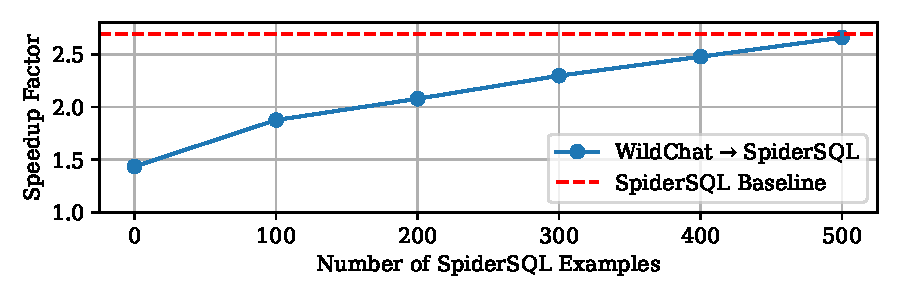
\includegraphics[width=\columnwidth,trim={5 5 5 5},clip]{figures/distribution_shift_speedup.pdf}
\end{subfigure}
\begin{subfigure}{0.5\columnwidth}
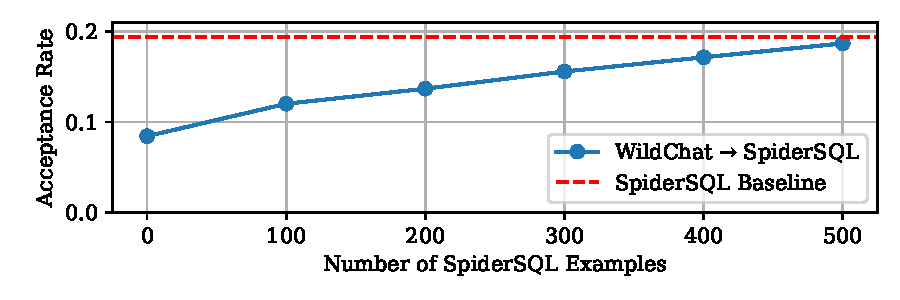
\includegraphics[width=\columnwidth,trim={5 5 5 5},clip]{figures/distribution_shift_acceptance.pdf}
\end{subfigure}
\caption{The performance of SuffixDecoding under input distribution shift. SuffixDecoding was trained on outputs from WildChat, while being evaluated on SpiderSQL. X axis: the number of SpiderSQL inputs, which are added to the global suffix tree after they are processed. Red line: the performance of SuffixDecoding if trained on 500 output examples from only SpiderSQL offline.} 
\label{fig:distribution-shift}
\end{figure}

\subsubsection{Predicting SuffixDecoding Effectiveness}
\label{sec:measuring-entropy}

SuffixDecoding tends to perform better on more structured tasks compared to very open-ended ones (e.g., AgenticSQL vs WildChat). We can measure this "structuredness" using empirical entropy. The steps are as follows: (1) create a suffix tree from example model outputs (100 examples is typically enough), (2) calculate the entropy of each node’s output distribution by determining how often each child node is accessed, and (3) compute a weighted average of this entropy across all nodes. A low average entropy indicates that output tokens are more predictable based on their prefixes, which generally suggests that Suffix Decoding will perform better.

\begin{table}[htbp]
\caption{Measured empirical entropy of our various evaluation datasets.}
\label{tab:entropy}
\small
\centering
\begin{tabular}{lc}
\toprule
Dataset & Average Entropy \\
\midrule
AgenticSQL (Enrich)   & 0.171 \\
AgenticSQL (Classify) & 0.738 \\
AgenticSQL (Extract)  & 0.0862 \\
AgenticSQL (SQL1)     & 1.52 \\
AgenticSQL (SQL2)     & 1.49 \\
AgenticSQL (SQL3)     & 1.51 \\
AgenticSQL (Combine)  & 1.49 \\
Spider                & 2.50 \\
WildChat              & 3.43 \\
Magicoder             & 2.95 \\
\bottomrule
\end{tabular}
\end{table}

Table~\ref{tab:entropy} shows the empirical entropy measured on samples from each of our evaluation datasets. We find that the average entropy is closely related to the intuitive understanding of the "structuredness" of each dataset. Additionally, it correlates well with the performance of SuffixDecoding on those datasets. Therefore, practitioners can calculate this value using a small number of output examples to assess whether SuffixDecoding is appropriate for their specific tasks.



\section{Scalability and Memory Overhead}
\label{sec:scalability-and-memory-overhead}

The suffix trees employed by Suffix Decoding are highly time and memory efficient. Table~\ref{tab:scalability} shows the per-token lookup time, update time, and memory consumption across various tree sizes (using requests from the SWE-Bench dataset). 

\begin{table}[h]
\centering
\caption{Performance metrics for different entry counts}
\label{tab:scalability}
\begin{tabular}{ccccc}
\toprule
Total \# entries & Total \# tokens & Memory footprint & Avg update time & Avg lookup time \\
                 &                 & (MB)             & per token ($\mu s$)  & per speculated token ($\mu s$) \\
\midrule
1 K entries & 27 M & 1670 MB & 3.95 & 12.18 \\
5 K entries & 143 M & 2980 MB & 4.06 & 10.93 \\
10 K entries & 285 M & 4070 MB & 4.05 & 12.00 \\
15 K entries & 429 M & 5110 MB & 4.07 & 11.62 \\
20 K entries & 572 M & 6150 MB & 4.04 & 11.64 \\
\bottomrule
\end{tabular}
\end{table}

Overall, the total memory consumption scales linearly with the size of the tree, and both the update and lookup times remain fast even with larger trees. Given typical server configurations, SuffixDecoding can cache many weeks of generated tokens before hitting CPU memory limits. For example, optimized inference engines running Llama-8B on an A100 GPU can typically generate $\sim 5000$ tokens per second (\citep{yin2024sglang}) or $\sim 432 M$ tokens per day. Typical A100 systems (e.g. AWS p4d.24xlarge) have 144GB of CPU memory per A100 GPU. This means that Suffix Decoding can potentially cache 31 days (see math below) of generated tokens per A100 GPU before hitting CPU memory limits. Beyond this limit, it is also straightforward to incorporate cache eviction (e.g. LRU) into Suffix Decoding to avoid out-of-memory problems.

\textbf{Time to fill up GPU memory:}
\begin{enumerate}
    \item Memory per token: $6.15~\text{GB} \div 572\text{M tokens} = 1.075 \times 10^{-8}~\text{GB/token}$
    \item Total token capacity: $144~\text{GB} \div (1.075 \times 10^{-8}~\text{GB/token}) = 1.34 \times 10^{10}~\text{tokens}$
    \item Time to fill: $(1.34 \times 10^{10}~\text{tokens}) \div (5000~\text{tok/s}) = 2.68 \times 10^{6}~\text{seconds} = \mathbf{31.0~\text{days}}$
\end{enumerate}

\subsection{Hybrid Fallback Threshold Sensitivity Analysis}
\label{sec:threshold-sensitivity}

The hybrid SuffixDecoding approach uses a fallback threshold $\tau$ to determine when to use suffix-tree-based speculation versus falling back to a model-based speculator (e.g., EAGLE-3). This section analyzes the sensitivity of performance to different threshold values across both open-ended and agentic workloads.

Table~\ref{tab:threshold-specbench} shows the wall-clock speedup results on Spec-Bench for various threshold values. For open-ended generation tasks, we find that setting $\tau$ close to or slightly exceeding the mean accepted tokens (MAT) of the model-based speculator yields the best performance. For instance, EAGLE-3 achieves a MAT of approximately 4.65 tokens/step on Spec-Bench. The results show that $\tau \in [5, 7]$ produces the highest overall speedups (2.5×), with performance being relatively stable across this range.

\begin{table}[h]
\centering
\caption{Hybrid SuffixDecoding speedup on Spec-Bench across different threshold values $\tau$.}
\label{tab:threshold-specbench}
\small
\begin{tabular}{lccccccc}
\toprule
$\tau$ & coding & qa & math & reasoning & stem & writing & Overall \\
\midrule
7 & 3.44 & 2.40 & 3.14 & 2.50 & 2.87 & 2.83 & 2.50 \\
6 & 3.19 & 2.22 & 2.88 & 2.30 & 2.68 & 2.61 & 2.31 \\
5 & 3.25 & 2.28 & 2.70 & 2.35 & 2.74 & 2.70 & 2.37 \\
4 & 3.07 & 2.22 & 2.72 & 2.25 & 2.57 & 2.64 & 2.25 \\
3 & 2.88 & 2.09 & 2.54 & 2.10 & 2.39 & 2.50 & 2.13 \\
2 & 2.73 & 2.04 & 2.40 & 2.01 & 2.19 & 2.36 & 2.03 \\
1 & 2.28 & 1.86 & 2.01 & 1.69 & 1.90 & 2.12 & 1.80 \\
0 (suffix only) & 1.83 & 1.77 & 1.97 & 1.39 & 1.39 & 1.33 & 1.66 \\
\bottomrule
\end{tabular}
\end{table}

Conversely, Table~\ref{tab:threshold-agenticsql} shows results for AgenticSQL, a highly repetitive agentic workload. Here, the standalone SuffixDecoding ($\tau = 0$) achieves the best overall speedup ($5.35\times$), as it can confidently speculate much longer sequences than model-based methods. Higher threshold values progressively degrade performance as the system increasingly falls back to less effective model-based speculation.

\begin{table}[h]
\centering
\caption{Hybrid SuffixDecoding speedup on AgenticSQL across different threshold values $\tau$.}
\label{tab:threshold-agenticsql}
\small
\begin{tabular}{lcccccc}
\toprule
$\tau$ & Classify & Extract & Enrich & Combine & SQL & Overall \\
\midrule
0 (suffix only) & 3.02 & 9.85 & 10.41 & 4.85 & 3.09 & 5.35 \\
1 & 2.31 & 7.03 & 8.37 & 3.38 & 2.17 & 3.95 \\
2 & 2.24 & 7.14 & 7.97 & 3.33 & 2.29 & 3.80 \\
3 & 2.22 & 5.51 & 5.68 & 3.52 & 2.20 & 3.22 \\
7 & 2.06 & 6.79 & 7.10 & 3.44 & 2.29 & 3.66 \\
\bottomrule
\end{tabular}
\end{table}

In summary, practitioners should set $\tau \approx \text{MAT}_{\text{fallback}}$ for mixed or open-ended workloads, where $\text{MAT}_{\text{fallback}}$ is the mean accepted tokens of the fallback model-based speculator. For highly repetitive agentic workloads, using SuffixDecoding alone ($\tau = 0$ or very low values) yields the best performance.

\section{Batch-level Speculation Control}
\label{sec:batch-speculation}

For batched serving scenarios, optimizing the speculation per request in a batch is crucial for many practical online deployments. While SuffixDecoding focuses on \textit{what} tokens to speculate, it is also compatible with existing works that explore \textit{how much} to speculate per request. For example, TurboSpec~\citep{liu2024turbospec} uses a "goodput" metric to balance speculation lengths and batch size, noting that optimal speculation decreases as batch size increases. AdaServe~\citep{adaserve} formulates multi-SLO serving as a constrained 
optimization problem and introduces SLO-customized speculative decoding that constructs speculation trees tailored to each request's latency target.
%
By dynamically adjusting the number of speculative tokens generated by the SuffixTree per request, SuffixDecoding can be integrated with TurboSpec to maximize the batch-wise goodput metric.
%
Furthermore, the statistics-based scoring used by Suffix Decoding can potentially better inform methods like TurboSpec. For example, choosing to speculate more from sequences that have a higher marginal score. 
%
These are interesting and important directions for future work.


